\documentclass{article}
\usepackage[utf8]{inputenc}

\title{Lecture 12: unsupervies learnring }
\author{wbg231 }
\date{November 2022}
\usepackage{tikz,graphicx,amsmath,amsfonts,amscd,amssymb,bm,cite,epsfig,epsf,url}
\begin{document}

\maketitle

\section{dimensionality reduction}
\begin{itemize}
\item 
%\item 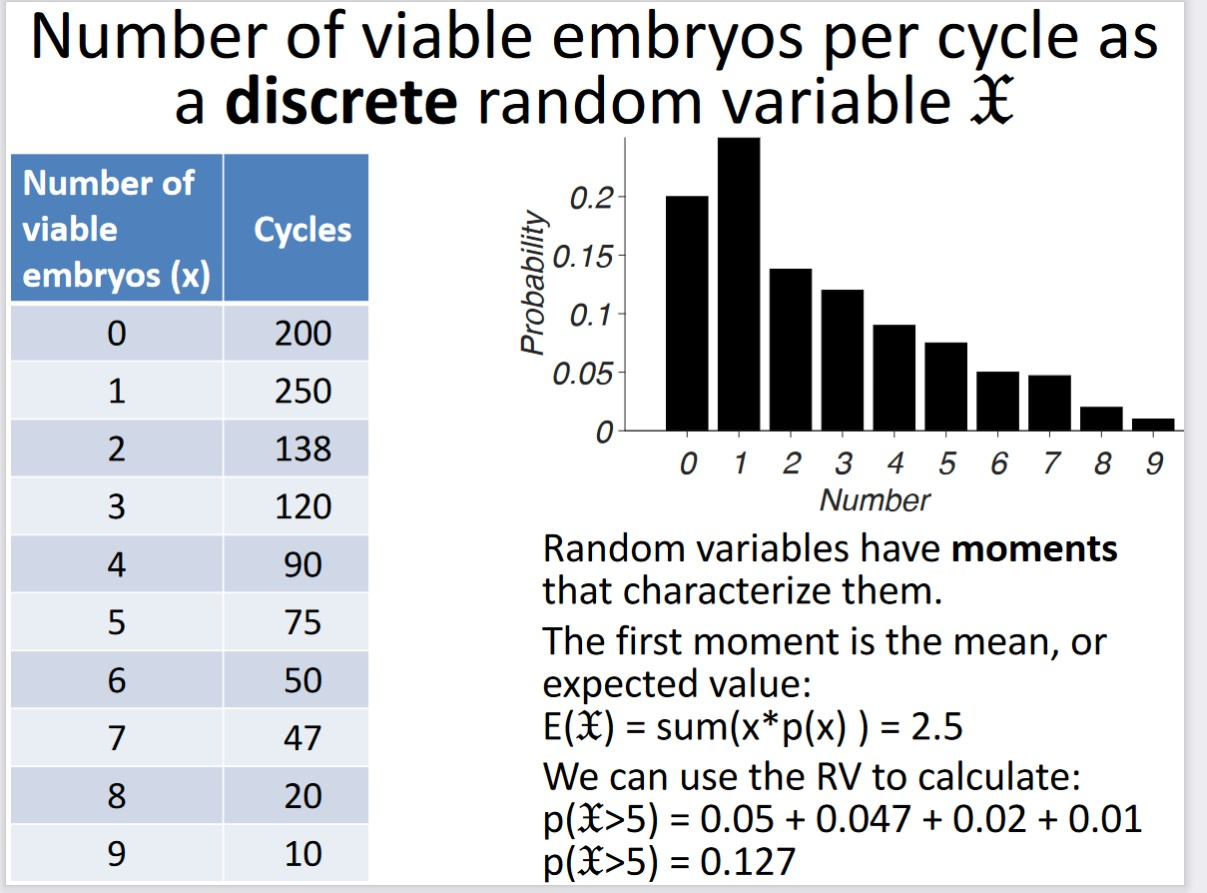
\includegraphics[width=7.5cm]{Final_Review/Lecture_2/lecture_1example.jpg}
\item in a highly multivariate dataset, could do something like lasso selection to find features
\item but instead of selecting features we could do something like clustering which allows us to not lose features 
\subsection{taking correlated information into account}
\item the point of commonality reduction is it takes a highly dimensional but dependant dataset in and outputs a lower dimensional but independent data set 
\item this is closer to feature extraction, we are finding new directions that contain a lot of variance, but not just selecting a few columns that we want 
\item if the correlation between the 40, 40 variables is independent we would see random correlation matrix 
\item but if there is some structure in our correlation matrix, the the PCA will not be random 
\item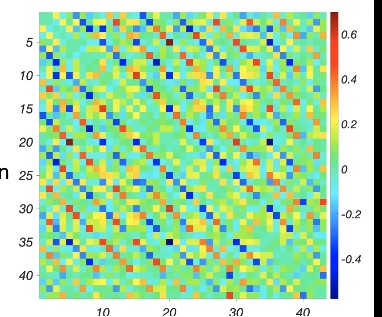
\includegraphics[width=5cm]{Final_Review/lecture_12/corealtion .jpg}
\item so this is a matrix that would lend its self well to PCA. 
\item the PCA only works if our data is standard normal 
\item can decompose any matrix using SVD
\subsection{SVD for image compression}
\item we have a picture of the Washington monument it is a high resolution image, we want to reduce the dimensions of this matrix
\item there are 324 component's of this matrix, in the SVD the singular values are decreasing in order of magnitude, so we just need the first however meant
\item with just the first 5 component's, it captures a lot of the image, but then there are diminishing returns to more eigen values 
\item within about 10\% of the information contains the signal 
\subsection{PCA}
\item PCA find an interpret able basis for our matrix 
\item first computes the covariance matrix 
\item the eigenvectors of the covariance matrix are the basis of the orthogonal basis 
\item we find the eigenvector hat is projected onto would max the variance 
\item we call that the first principle component, then the second principle component is orthogonal to that 
\item so he we can express our data in far fewer dimensions 
\item we put in an n dimensional dataset and what comes out is an n dimension dataset of eigenvectors that are orthogonal to one another 
\item PCA can always produce n orthogonal eigenvectors 
\subsection{pca what is the point}
\item we can just keep a few eigenvectors that account for some large quantity of the variance in the data
\item think of feature extraction as rotation 
\subsection{typcial ml work flow}
\item start with multivariate data
\item use dimensional reduction method, if you reduce it to 1 dimension then do simple classification 
\item otherwise we have to do some classification \subsection{example}
\item we want to find out what students are depressed.
\item it matters if we are able to intervene early
\item we get a pca with a large elbow plot that tells us to keep approximately 2 eigen vectors 
\item we can see in the code section to see how to interpret them 
\item the pca will rotate our data in terms of the important features.
\subsection{clustering}
\item we are basscially looking 
\end{itemize}

\end{document}
